\section{Internship Description}

\subsection{Internship experience overview}

    \subsubsection{Workplace}
    The office in which I was employed is situated in the Etown Building, located at 364 Cong Hoa Street, Ward 13, Tan Binh District, Ho Chi Minh City, Vietnam. The building is well-appointed with modern amenities, including a high-quality lighting system conducive to visual comfort, ergonomic chairs, solid desks, and high-speed internet access. My designated workspace was in the "Talent pool" area of the floor, where all interns were assigned. For professional purposes, I was provided with a high-specification desktop computer to facilitate my work.

        
    \subsubsection{Language and formal communication}
    Within the professional environment, I employed both English and Vietnamese for interpersonal communication. Given that the majority of my colleagues were Vietnamese, I primarily used Vietnamese for information sharing. However, in regard to the reporting procedures and written documents, it was explicitly mandated that the reports be composed in the English language.
    
    \subsubsection{The project team}
    Our team comprises three members, each assigned specific roles that contribute to the project's success. We follow the Agile software development methodology, which defines roles such as Product Owners, Team Lead, and Development Team. Given the limited team size, I assume dual responsibilities, functioning both as the Team Lead and as a member of the Development Team (Backend developer).

    \subsubsection{Project specification and process}
    
    The internal project's objective is to build a web application which helps managers monitor the monthly efforts of each employee, plan and report the billing information list. This involves a comprehensive understanding of the requirements, the billing data and the structure of all components. It requires us to analyse the requirements and application backlog carefully and collaborate closely with the Product Owner as well as the Customer.

    To effectively fulfill these responsibilities, we adhere to the Agile software development methodology, as previously outlined. Our team employs a standardized approach that centers on three primary domains: analysis, implementation, and reporting. Each sprint is scheduled on a weekly basis, with the team dedicating their efforts to achieving the sprint goal until its conclusion. Upon completion of the sprint, we conduct a two-hour meeting during which we discuss task progress, completed work, encountered challenges, and plans for the subsequent sprint.
    
    \subsubsection{Team communication}

    \begin{tabular}{ @{} m{0.25\textwidth} m{0.7\textwidth} @{} }
      \begin{minipage}{\linewidth}
        \centering
        
\includegraphics[width=0.7\linewidth]{graphics/ms-teams-logo.jpg}
        \captionof{figure}{Microsoft Teams platform}
        \label{fig:ms-teams-logo}
      \end{minipage}
      &
      \begin{minipage}{\linewidth}
            For communication with each other in a team, we use Microsoft Teams platform.  Moreover, it is imperative that employees are assigned to specific channels within Slack that align with their respective tasks and responsibilities in the workplace. This ensures a streamlined and efficient flow of information, facilitates task-related discussions and collaborations, and contributes to the overall effectiveness and productivity within the organizational framework.
      \end{minipage}
    \end{tabular}

    
    \subsubsection{Task assignment}
 %    \begin{figure}[H]
	% 		\centering
	% 		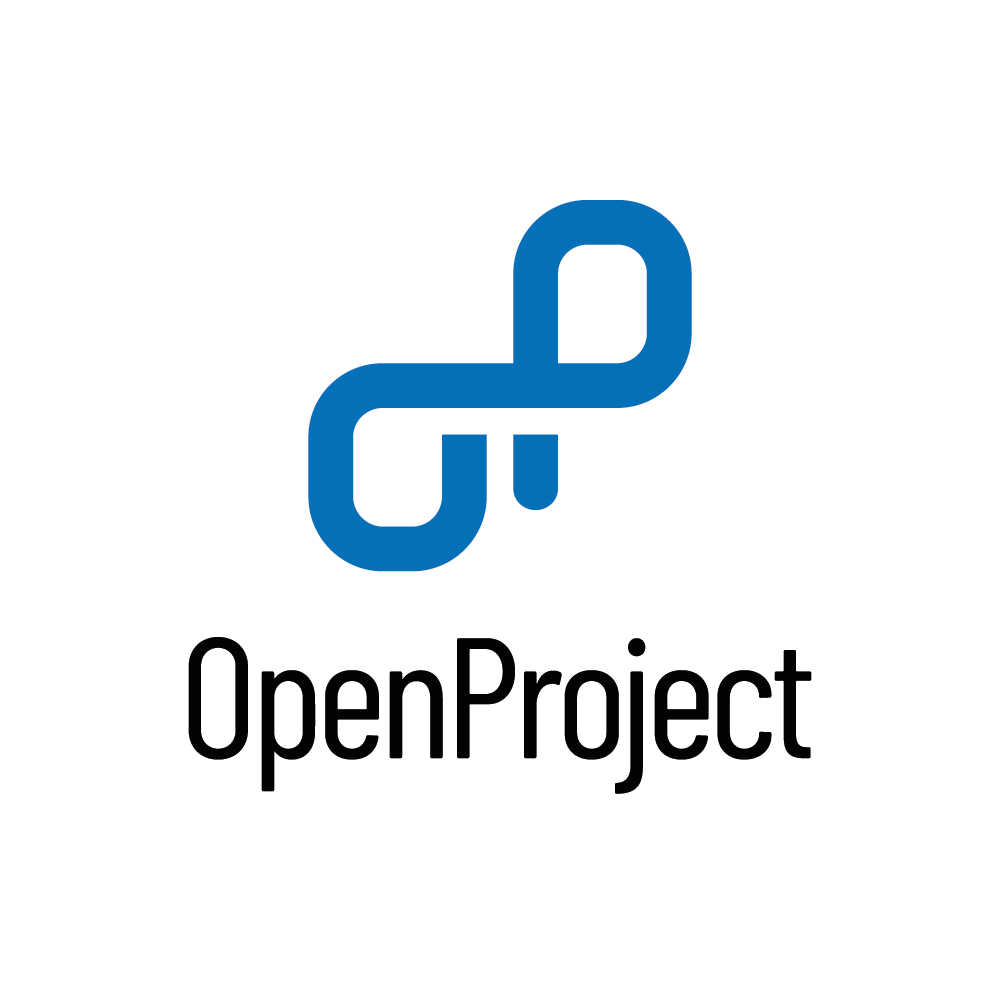
\includegraphics[scale=0.2]{graphics/openproject-logo.png}
	% 		\caption{OpenProject project management platform}
	% 		\label{fig:openProject}
	% \end{figure}
    \begin{figure}[H]
        \centering
        \begin{minipage}{.5\textwidth}
          \centering
          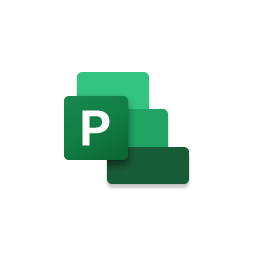
\includegraphics[width=.4\linewidth]{graphics/ms-project.png}
          \captionof{figure}{Microsoft Project}
          \label{fig:msProject}
        \end{minipage}%
        \begin{minipage}{.5\textwidth}
          \centering
          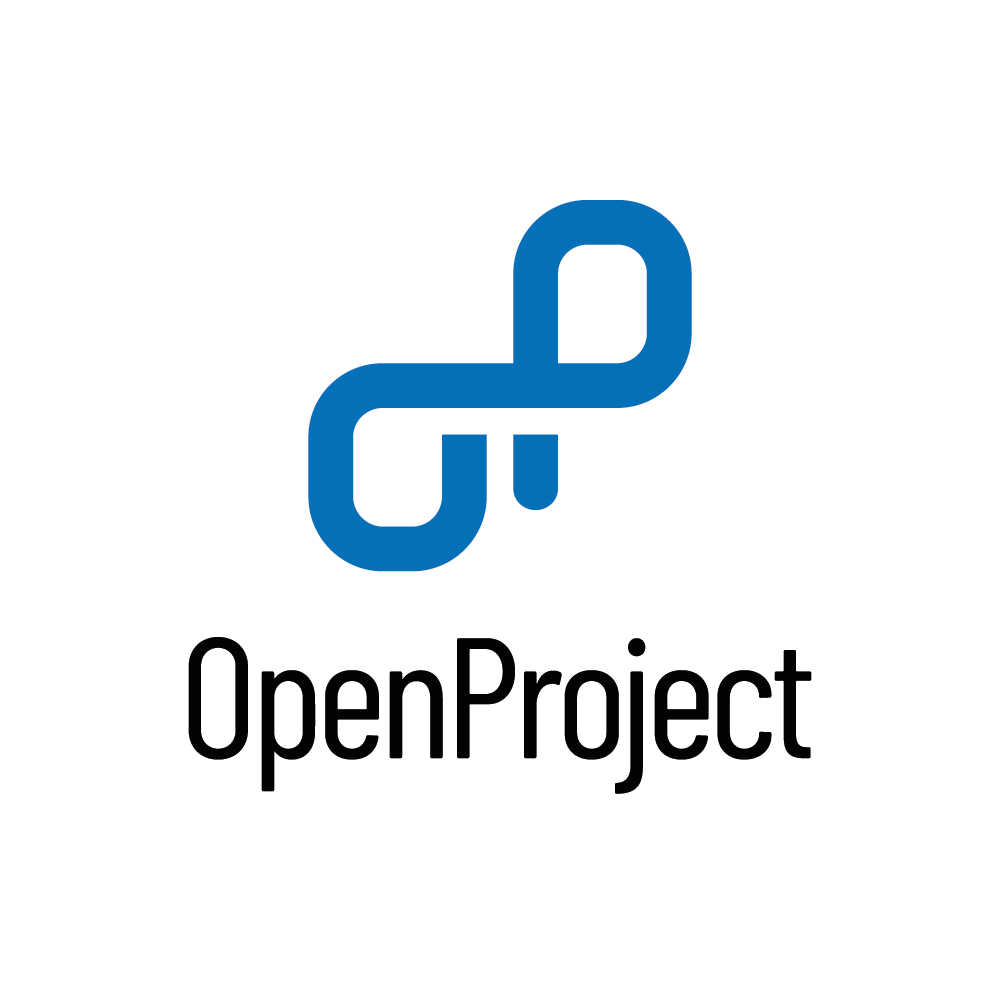
\includegraphics[width=.4\linewidth]{graphics/openproject-logo.png}
          \captionof{figure}{OpenProject}
          \label{fig:openProject}
        \end{minipage}
    \end{figure}

    In the training phase, I was assigned tasks on the Microsoft Project board by my manager. I had to follow the schedule to complete the training tasks. The structure of the task board based on the waterfall project management framework, means that I have to complete the previous task to do the next one. The schedule, in general is well-defined, and I can follow the timeline smoothly. \\
    
    The reason why Microsoft Project platform is used is that it is a robust project management software developed by Microsoft, widely utilized across various industries for its comprehensive tools that facilitate project planning, scheduling, resource allocation, and progress tracking. One of its primary advantages is its ability to manage complex projects with multiple interconnected tasks through Gantt charts, which provide a visual timeline of project activities and dependencies. This feature allows project managers to effectively schedule tasks, allocate resources, and identify potential bottlenecks. \cite{ms_project}\\

    
    When being deployed to the internal project, to ensure effective task allocation, it is imperative that business owners clearly define the due dates for each task. Hence, the platform that is utilized is Open Project. \\
    OpenProject is a web-based project management software that offers several advantages for task assignment in web application projects. Here are the key benefits and steps involved:
    \begin{enumerate}
        \item \textbf{Single Source of Information:} OpenProject serves as a centralized platform, providing project members with access to tasks, responsibilities, and timings from anywhere. This feature is particularly useful for remote teams, allowing collaboration across hierarchies and departments. \cite{why_openproject}

        \item \textbf{Clear Responsibilities:} With OpenProject, you can clearly define responsibilities for each team member. Whether they work within the same team or across different units, everyone can access project-related information easily.
    \end{enumerate}
    \noindent As a team leader of the internal project, I had to manage and assign tasks to each member based on their roles. By pointing out the main phases clearly, I can then define features (based on user stories) for each phase, and schedule the implementation for each member.

    
    

\subsection{Working tools}
    \subsubsection{Operating systems}

    \begin{figure}[H]
			\centering
			
\includegraphics[scale=0.2]{graphics/ubuntu-server-logo.png}
			\caption{Ubuntu Server}
			\label{fig:ubuntuServer}
	\end{figure}
    
    Ubuntu Server is a widely-used, open-source operating system tailored for servers, developed and maintained by Canonical Ltd. Based on Debian, Ubuntu Server offers robust security features, extensive software repositories, and a stable platform for running server applications.
    
    \noindent Its key advantages include ease of use, especially with its user-friendly installation process and extensive documentation, making it accessible even to those new to Linux. It supports a variety of architectures and integrates well with cloud platforms like AWS, Azure, and Google Cloud, offering scalability and flexibility. Additionally, its regular Long Term Support (LTS) releases ensure sustained updates and security patches for up to five years. However, Ubuntu Server has its drawbacks. It may require more frequent updates and patches compared to some other server OS options, potentially leading to higher maintenance. \cite{ubuntu_server}

    Therefore, we choose Ubuntu Server as our main development environment.    
    
    \subsubsection{Integrated Development Environment}

    \begin{figure}[H]
			\centering
			
\includegraphics[scale=0.1]{graphics/vscode-logo.jpg}
			\caption{Visual Studio Code}
			\label{fig:vsCode}
	\end{figure}
    
    Visual Studio Code (VS Code) is a free, open-source Integrated Development Environment (IDE) developed by Microsoft, widely adopted by developers for its versatility and robust feature set. Besides that, it supports macOS, Linux, and Windows, making it accessible across platforms. \cite{why_vscode} Here are the reasons why we make use of VS Code for web application development:

    \begin{enumerate}
        \item \textbf{Lightweight and Fast:} VS Code is lightweight and performs exceptionally well, even on less powerful devices. Its efficient design ensures a smooth edit-build-debug cycle, allowing developers to focus on their ideas without distractions. 

        \item \textbf{Rich Language Support:} With support for hundreds of languages, VS Code provides syntax highlighting, auto-indentation, and bracket matching. It also includes IntelliSense code completion, semantic understanding, and navigation, enhancing productivity. \cite{why_vscode}

        \item \textbf{Built-in Web Technologies:} VS Code offers excellent tooling for web development, including support for JavaScript, TypeScript, JSX/React, HTML, CSS, SCSS, Less, and JSON. Its integration with Git simplifies source control tasks within the editor. \cite{why_vscode}
        
    \end{enumerate}

    \subsubsection{Back-end framework}
    \begin{figure}[H]
        \centering
        \begin{minipage}{.5\textwidth}
          \centering
          
\includegraphics[width=.25\linewidth]{graphics/python-logo.png}
          \captionof{figure}{Python programming language}
          \label{fig:python}
        \end{minipage}%
        \begin{minipage}{.5\textwidth}
          \centering
          
\includegraphics[width=.65\linewidth]{graphics/flask-logo.png}
          \captionof{figure}{Flask web framework}
          \label{fig:flask}
        \end{minipage}
    \end{figure}

    The internal web application project is built based on the Flask framework (a micro web framework written in Python). We chose this framework for the project since Flask follows a minimalist approach, allowing developers to build web applications without unnecessary components. Its lightweight design ensures swift load times and efficient resource utilization.\cite{why_flask}. Besides that, Flask integrates well with other Python libraries, enabling us to add features like authentication, databases, and form handling.


    \subsubsection{Databases management system} \label{Databases management system}
    \begin{figure}[H]
			\centering
			
\includegraphics[scale=0.15]{graphics/mysql-logo.png}
			\caption{MySQL database management system}
			\label{fig:mySQL}
	\end{figure}

     MySQL, an open-source relational database management system (RDBMS), offers several compelling advantages for web applications. As a widely adopted choice, MySQL delivers blazing-fast performance, making it a preferred option for high-traffic web services. Its efficient query execution and optimized indexing contribute to its outstanding speed. \cite{why_mysql} In addition, MySQL supports replication, clustering, and failover mechanisms, ensuring data availability and fault tolerance. It can handle large-scale deployments with ease. \cite{why_mysql_2}


    \subsubsection{Version control system}
    \begin{figure}[H]
        \centering
        \begin{minipage}{.5\textwidth}
          \centering
          
\includegraphics[width=.35\linewidth]{graphics/git-logo.png}
          \captionof{figure}{Git}
          \label{fig:git}
        \end{minipage}%
        \begin{minipage}{.5\textwidth}
          \centering
          
\includegraphics[width=.2\linewidth]{graphics/gitlab-logo.png}
          \captionof{figure}{Gitlab}
          \label{fig:gitlab}
        \end{minipage}
    \end{figure}
    Git, in general, is a version control system. It provides a centralized database to manage versions of files, eliminating the need for manual folder-based versioning. Git supports collaboration, easy backups, and flexible platforms. Meanwhile, GitLab is an extended version of version control. GitLab provides Integrated DevOps, Self-hosting, Branch Protection, and User-Friendly Package Distribution.
    
    Git and GitLab empower developers to collaborate efficiently, manage code, and streamline workflows. While Git handles version control, GitLab extends functionality with integrated tools and automation. 
    